\documentclass[12pt, a4paper]{article}
\usepackage[utf8]{vietnam}
\usepackage[margin = 2cm]{geometry}
\usepackage{amsmath,amsfonts,amssymb}
\usepackage{indentfirst,enumitem}
\usepackage{graphicx}
\usepackage[font=small,labelfont=bf]{caption}
\usepackage{multicol}
\usepackage{setspace}
\usepackage{hyperref}
\usepackage{listings}
\usepackage{tabularx}
\usepackage{hyperref}
\usepackage[dvipsnames]{xcolor}
\usepackage{scrextend}
\usepackage{comment}
\usepackage{soul}
\usepackage{tikz,tkz-tab}
\usepackage{lscape}
\usepackage{float,lscape}
\usepackage{fancyhdr}
\usepackage{tcolorbox}
\usepackage{titling}
\usepackage{import}
\usepackage{titlesec}
\usepackage{color}
%%%%%%%%%%%%%%%%%%%%

\hypersetup{
    colorlinks=true,% make the links colored
}

\pagestyle{fancy}
\fancyhead[r]{Huy Vu}
\fancyhead[c]{\bfseries PLĐC}
\fancyhead[l]{\today}
\renewcommand{\headrulewidth}{0.2pt}
\setlength{\headheight}{15pt}
\onehalfspacing

\begin{document}
\begin{titlepage}
    \centering
    \vspace*{1in}

    {\LARGE \bfseries PHÁP LUẬT VIỆT NAM ĐẠI CƯƠNG}\\[1.5cm]

    {\large Huy Vu}\\[0.5cm]
    {\large Faculty of Electrical and Electronics Engineering}\\
    {\large Ho Chi Minh City University of Technology}\\[2cm]

    {\large TP.Hồ Chí Minh - \today}

    \vfill
\end{titlepage}
{
  \hypersetup{linkcolor=[RGB]{236, 16, 145}}
  \tableofcontents
}
\newpage
\section{NHỮNG KHÁI NIỆM CHUNG VỀ NHÀ NƯỚC}
\subsection{NGUỒN GỐC, KHÁI NIỆM VÀ ĐẶC TRƯNG CỦA NHÀ NƯỚC}
Nhà nước là một tổ chức có quyền lực chính trị đặc biệt, có quyền quyết định cao nhất trong phạm vi lãnh thổ, thực hiện quản lý xã hội bằng pháp luật và bộ máy được duy trì bằng nguồn lực thuế đóng góp từ xã hội.

Bản chất của nhà nước: Tính giai cấp + Tính xã hội.

Đặc trưng của nhà nước:
\begin{itemize}
  \item Phân chia dân cư thành các đơn vị hành chính lãnh thổ và quản lý.
  \item Thiết lập quyền lực công cộng đặc biệt tách rời khỏi xã hội và áp đặt lên toàn xã hội.
  \item Có chủ quyền quốc gia.
  \item Quy định và thu thuế một cách bắt buộc.
  \item Ban hành pháp luật và xác lập trật tự pháp luật đối với toàn xã hội.
\end{itemize}
\subsection{BỘ MÁY NHÀ NƯỚC CỘNG HÒA XÃ HỘI CHỦ NGHĨA VIỆT NAM}
\noindent\textit{Bộ máy nhà nước:}
\begin{itemize}
  \item là hệ thống các cơ quan nhà nước từ trung ương xuống địa phương.
  \item được tổ chức theo những nguyên tắc chung thống nhất.
  \item tạo thành cơ chế đồng bộ để thực hiện các nhiệm vụ và chức năng của nhà nước.
\end{itemize}
\textit{Cơ quan nhà nước - bộ phận cấu thành của bộ máy nhà nước:}
\begin{itemize}
  \item là một tổ chức cấu thành bộ máy nhà nước.
  \item có tính chất, chức năng, nhiệm vụ, quyền hạn, cơ cấu tổ chức và hình thức khác nhau.
  \item có thể phân biệt với các tổ chức khác.
\end{itemize}
\subsubsection{NHỮNG NGUYÊN TẮC CƠ BẢN CỦA BỘ MÁY NHÀ NƯỚC CỘNG HOÀ XÃ HỘI CHỦ NGHĨA VIỆT NAM}
\textit{a. Nguyên tắc tất cả quyền lực nhà nước thuộc về Nhân dân:} Tất cả quyền lực nhà nước thuộc về Nhân dân. Quyền lực nhà nước do nhân dân, vì Nhân dân.

\textit{b. Nguyên tắc quyền lực nhà nước là thống nhất, có sự phân công, phối hợp, kiểm soát giữa các cơ quan nhà nước trong việc thực hiện quyền lập pháp, hành pháp, tư pháp:}
\begin{itemize}
  \item Khẳng định QLNN là \textbf{thống nhất}, không có sự phân chia, là Nhà nước của Nhân dân, do Nhân dân và vì Nhân dân.
  \item Quyền lực phải được \textbf{phân công} cho các cơ quan nhà nước thực hiện. 
  \item Các cơ quan nhà nước phải \textbf{phối hợp} với nhau trong việc thực hiện.
  \item Có cơ chế \textbf{kiểm soát} quyền lực
\end{itemize} 

\textit{c. Nguyên tắc Đảng lãnh đạo}

\textit{d. Nhà nước được tổ chức, hoạt động và quản lý xã hội bằng Hiến pháp và pháp luật}

\textit{e. Nguyên tắc tập trung dân chủ}
\subsubsection{Tổ chức và hoạt động của các cơ quan trong bộ máy Nhà nước Cộng hoà xã hội chủ nghĩa Việt Nam}
\begin{center}
  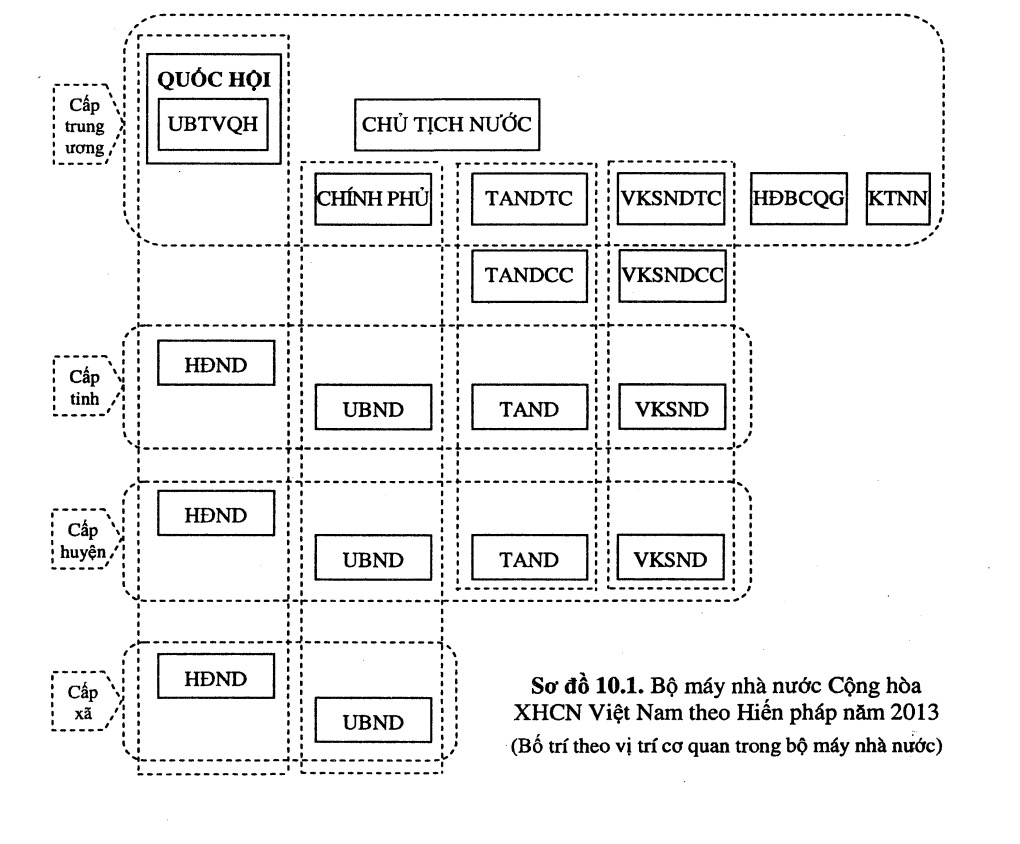
\includegraphics[width = 0.75\textwidth]{./image/3.png}\\
  Đảng là tổ chức chính trị
\end{center}

Hệ thống chính trị là một cơ cấu bao gồm Nhà nước, các Đảng phái, các Đoàn thể, các tổ chức chính trị-xã hội tồn tại và hoạt động trong khuôn khổ pháp luật hiện hành, được chế định theo tư tưởng giai cấp cầm quyền, nhằm tác động vào các quá trình kinh tế-xã hội với mục đích duy trì và phát triển chế độ đó.

\textit{a. Quốc hội:} là cơ quan đại biểu/đại diện cao nhất của Nhân dân, là cơ quan dân cử ở cấp trung ương, là cơ quan quyền lực nhà nước cao nhất. Quốc hội có 3 chức năng sau:
\begin{itemize}
  \item Thực hiện quyền lập hiến, lập pháp.
  \item Giám sát tối cao đối với hoạt động Nhà nước.
  \item Quyết định các vấn đề quan trọng của đất nước.
\end{itemize}
\begin{center}
  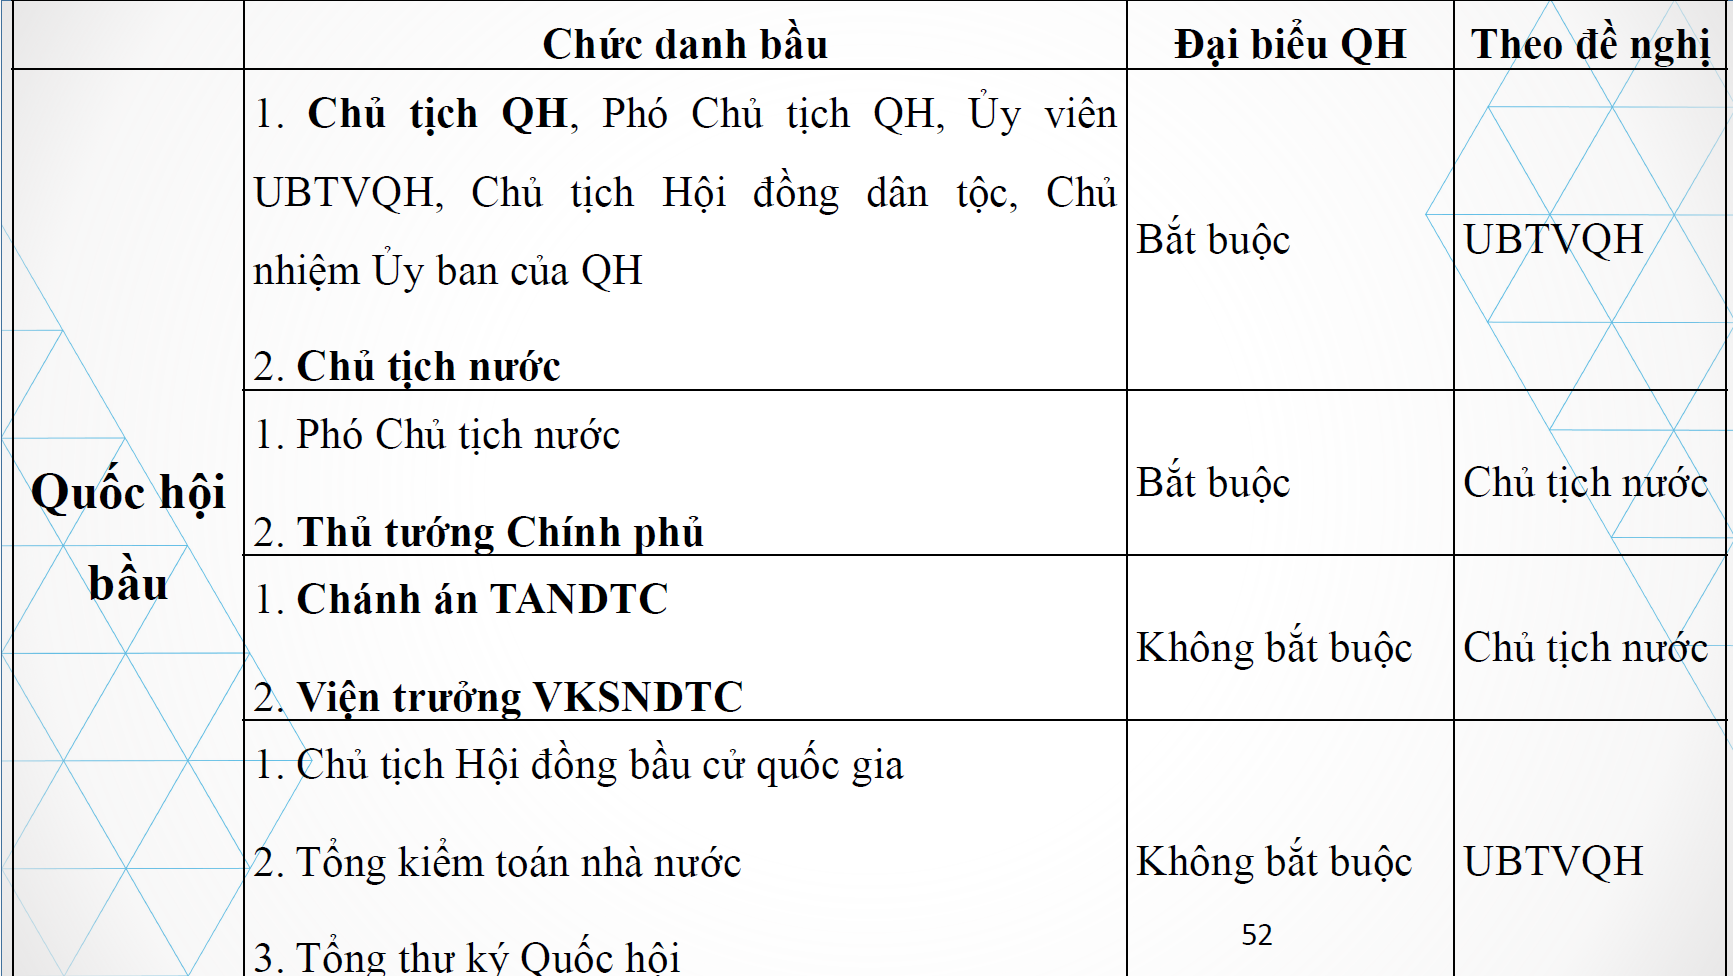
\includegraphics[width = 0.7\textwidth]{./image/4.png}
\end{center}
\begin{center}
  \textit{Cơ cấu tổ chức của Quốc hội}\\
  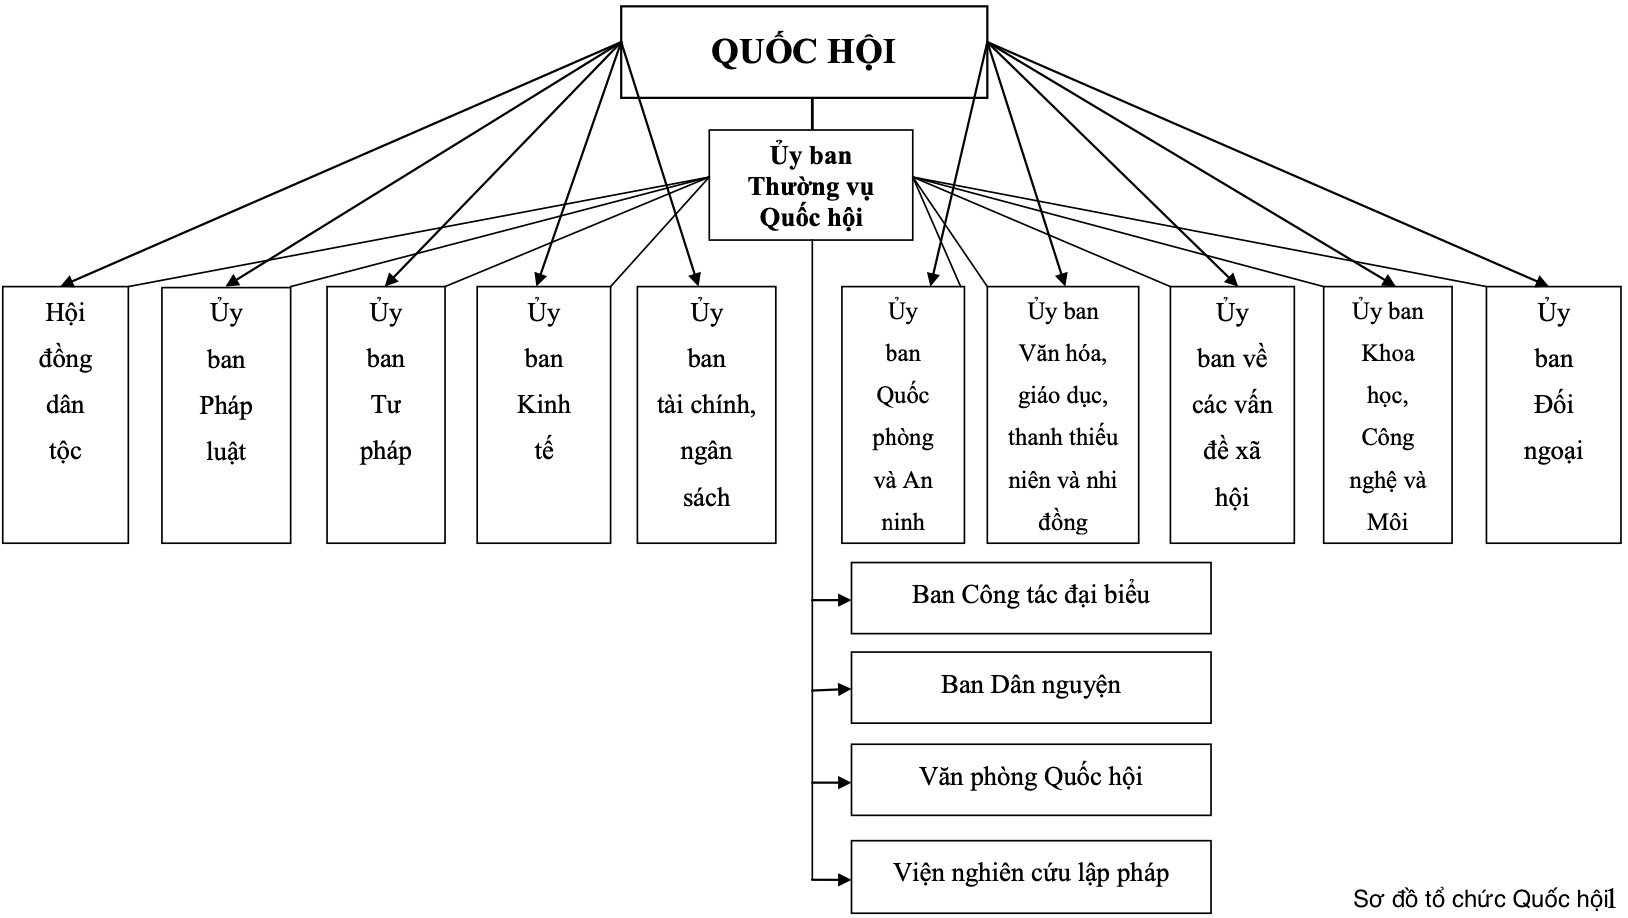
\includegraphics[width = 0.7\textwidth]{./image/5.png}
\end{center}

\textit{Hội đồng nhân dân:}
\begin{itemize}
  \item Là cơ quan quyền lực nhà nước ở cấp địa phương, là cơ quan dân cử ở cấp địa phương.
  \item Là cơ quan đại diện cho ý chí, nguyện vọng và quyền làm chủ của Nhân dân.
  \item HĐND là cơ quan duy nhất ở ĐP do cử tri ở ĐP trực tiếp bầu ra; HĐND là đại diện tiêu biểu nhất cho tiếng nói, ý chí của nhân dân ở ĐP.
  \item Chịu trách nhiệm trước Nhân dân ở địa phương và cơ quan nhà nước cấp trên.
\end{itemize}  

\textit{Chức năng của HĐND:}
\begin{itemize}
  \item Thứ nhất, quyết định những vấn đề của địa phương do luật quy định.
  \item Thứ hai, Hội đồng Nhân dân giám sát việc tuân thủ hiến pháp và pháp luật ở địa phương và việc thực hiện nghị quyết của Hội đồng Nhân dân.
\end{itemize}

\textit{b. Chủ tịch nước:} là người đứng đầu Nhà nước, thay mặt nước Cộng hòa xã hội chủ nghĩa Việt Nam về đối nội và đối ngoại.

\textit{c. Chính phủ:} là cơ quan hành chính nhà nước cao nhất của nước Cộng hòa xã hội chủ nghĩa Việt Nam. thực hiện quyền hành pháp, là cơ quan chấp hành của Quốc hội. Chức năng bao gồm: tổ chức thi hành Hiến pháp và pháp luật. Hoạch định chính sách quốc gia, trình dự án luật, pháp lệnh.

\textit{Ủy ban Nhân dân:} là cơ quan chấp hành của Hội đồng Nhân dân cùng cấp, là cơ quan hành chính nhà nước tại địa phương.

\textit{d. Tòa án Nhân dân:} cơ quan xét xử của nước Cộng hòa xã hội chủ nghĩa Việt Nam, thực hiện quyền tư pháp.
\begin{center}
  \textit{Cơ cấu tổ chức của Tòa án Nhân dân}\\
  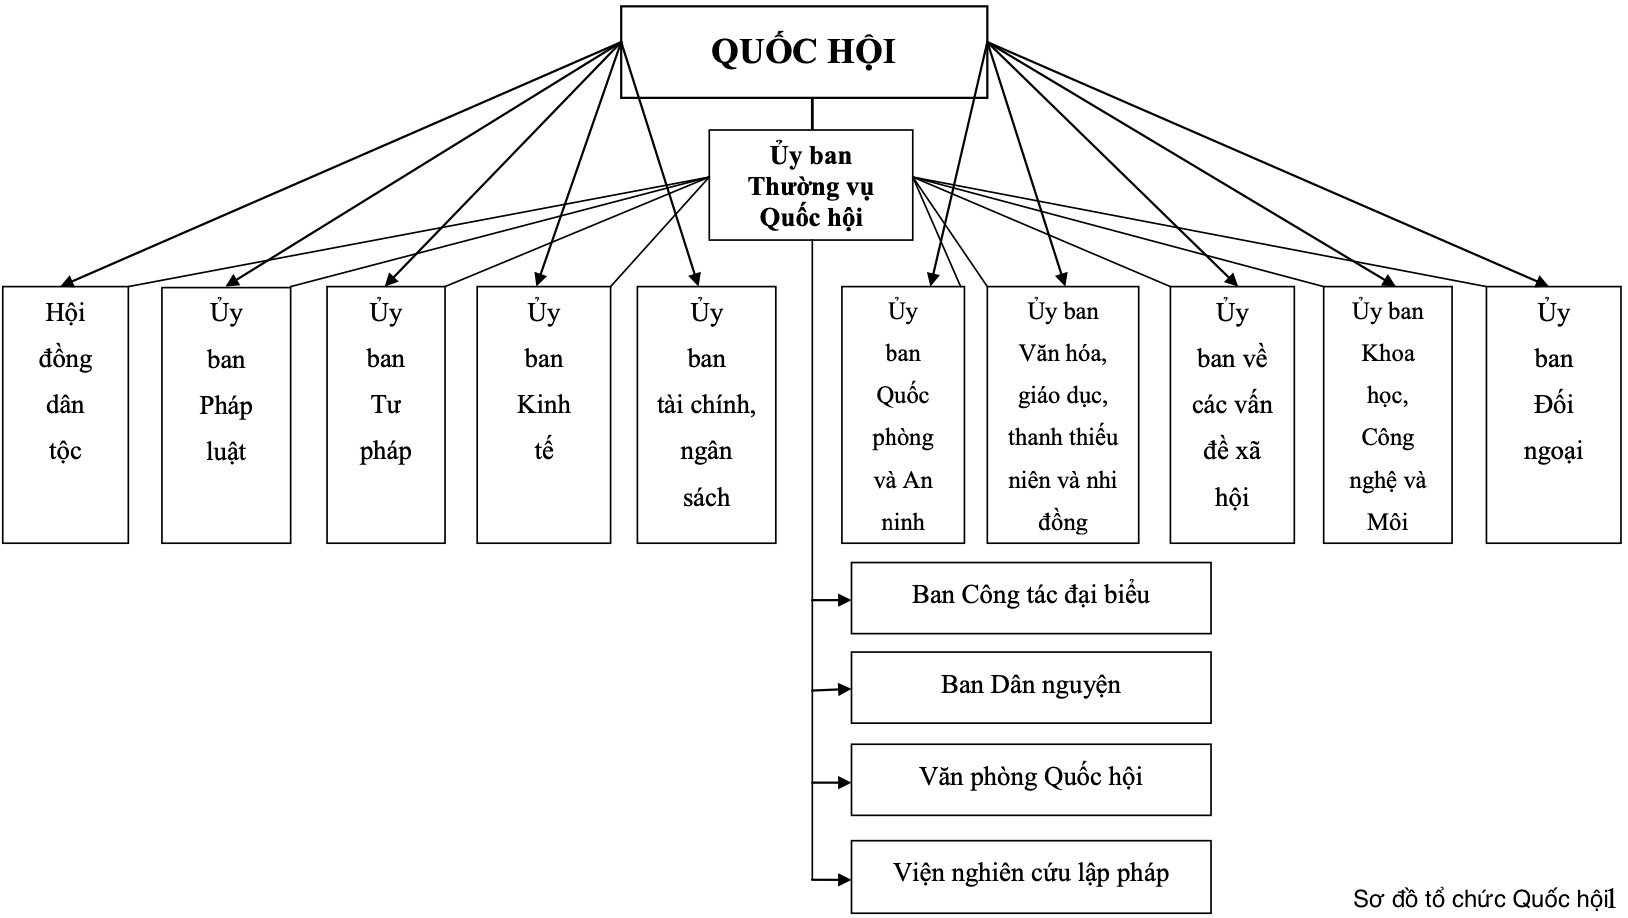
\includegraphics[width = 0.75\textwidth]{./image/5.png}
\end{center}

\textit{e. Viện kiểm soát Nhân dân:} thực hiện quyền công tố, kiểm soát hoạt động tư pháp.
\begin{center}
  \textit{Cơ cấu tổ chức của Viện kiểm soát Nhân dân}\\
  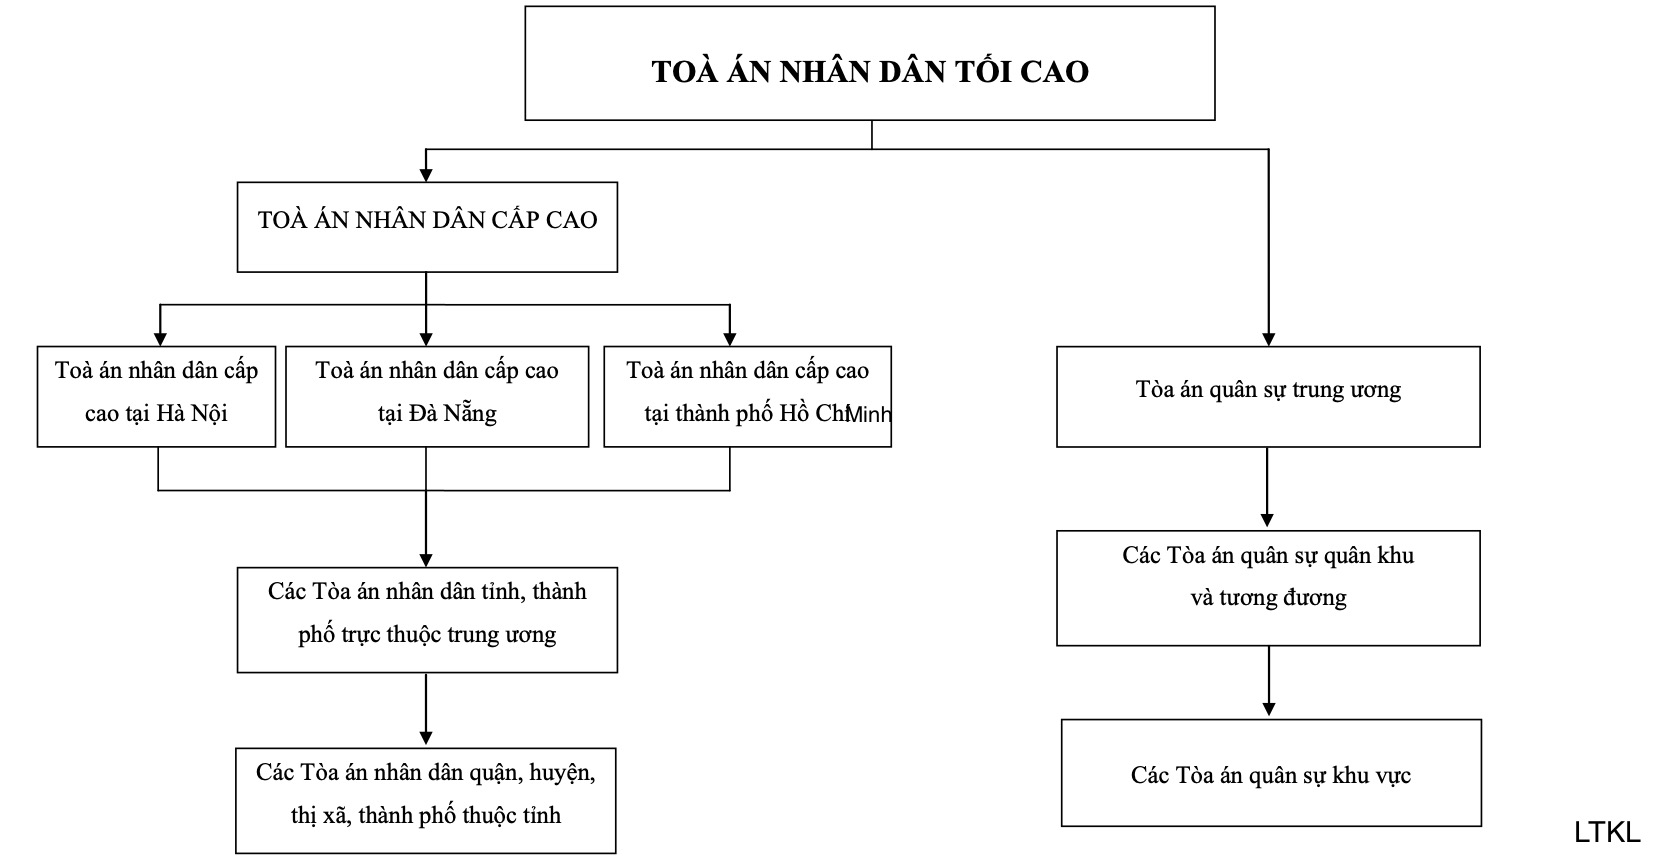
\includegraphics[width = 0.75\textwidth]{./image/6.png}
\end{center}
\end{document}